\chapter{Appendix}
This part is placed in the appendix because it adds complexity and is not absolutely necessary to understand the main ideas on the interoperability. 

\section{Merkle trees}
\subsection{Trie}
Binary merkle tree are used in bitcoin. 
In Ethereum a more complicated version is used, derived from the patricia trie. First let's understand what a trie is. 
\begin{figure}[H]
    \centering
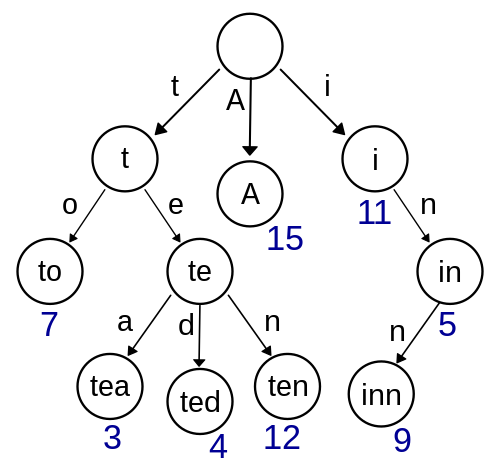
\includegraphics[width=0.3\linewidth]{background/trie.png}
    \caption{Trie representing the words "A", "to", "tea", "ted", "ten", "i", "in", and "inn"}
    \label{fig:trie}
\end{figure}
A trie is a tree data structure where the key of the node is also his path from the root. The key is usually a string.
In other words positions in the trie is determined directly from the key and the inverse is correct. 

Let's say you want to save n words in the trie:
\begin{enumerate}
    \item From the root, at step 1 we take the first letter of each of the n words and create a leaf for each different ones. In the example from the figure above, we  take A from A, t from to, tea, ted, ten, i from i, in and inn. We have then 3 nodes from the root: t, A, i
    \item at step t, repeat the first step but instead take the t first letters. 
    \item stop when all the original words are in a leaf. 
\end{enumerate}
If we have a string with 200 letters, we'll have to create 200 levels.
\subsection{Patricia trie}
As said in the last section, if you have a n length word you'll have to create n levels, which is not optimized in term of storage. 
Instead, radix tree and Patricia tree are a compressed version of the above trie.
\begin{figure}[H]
    \centering
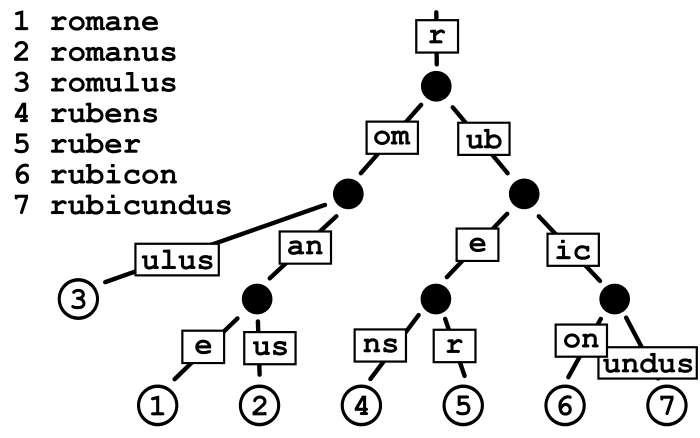
\includegraphics[width=0.4\linewidth]{background/patricia.png}
    \caption{Patricia tree}
    \label{fig:patricia}
\end{figure}
Here, we are not limited at each step in terms of length of the key.

\subsection{Patricia merkle tree}
\label{merkle:ethereum}
\begin{figure}[H]
    \centering
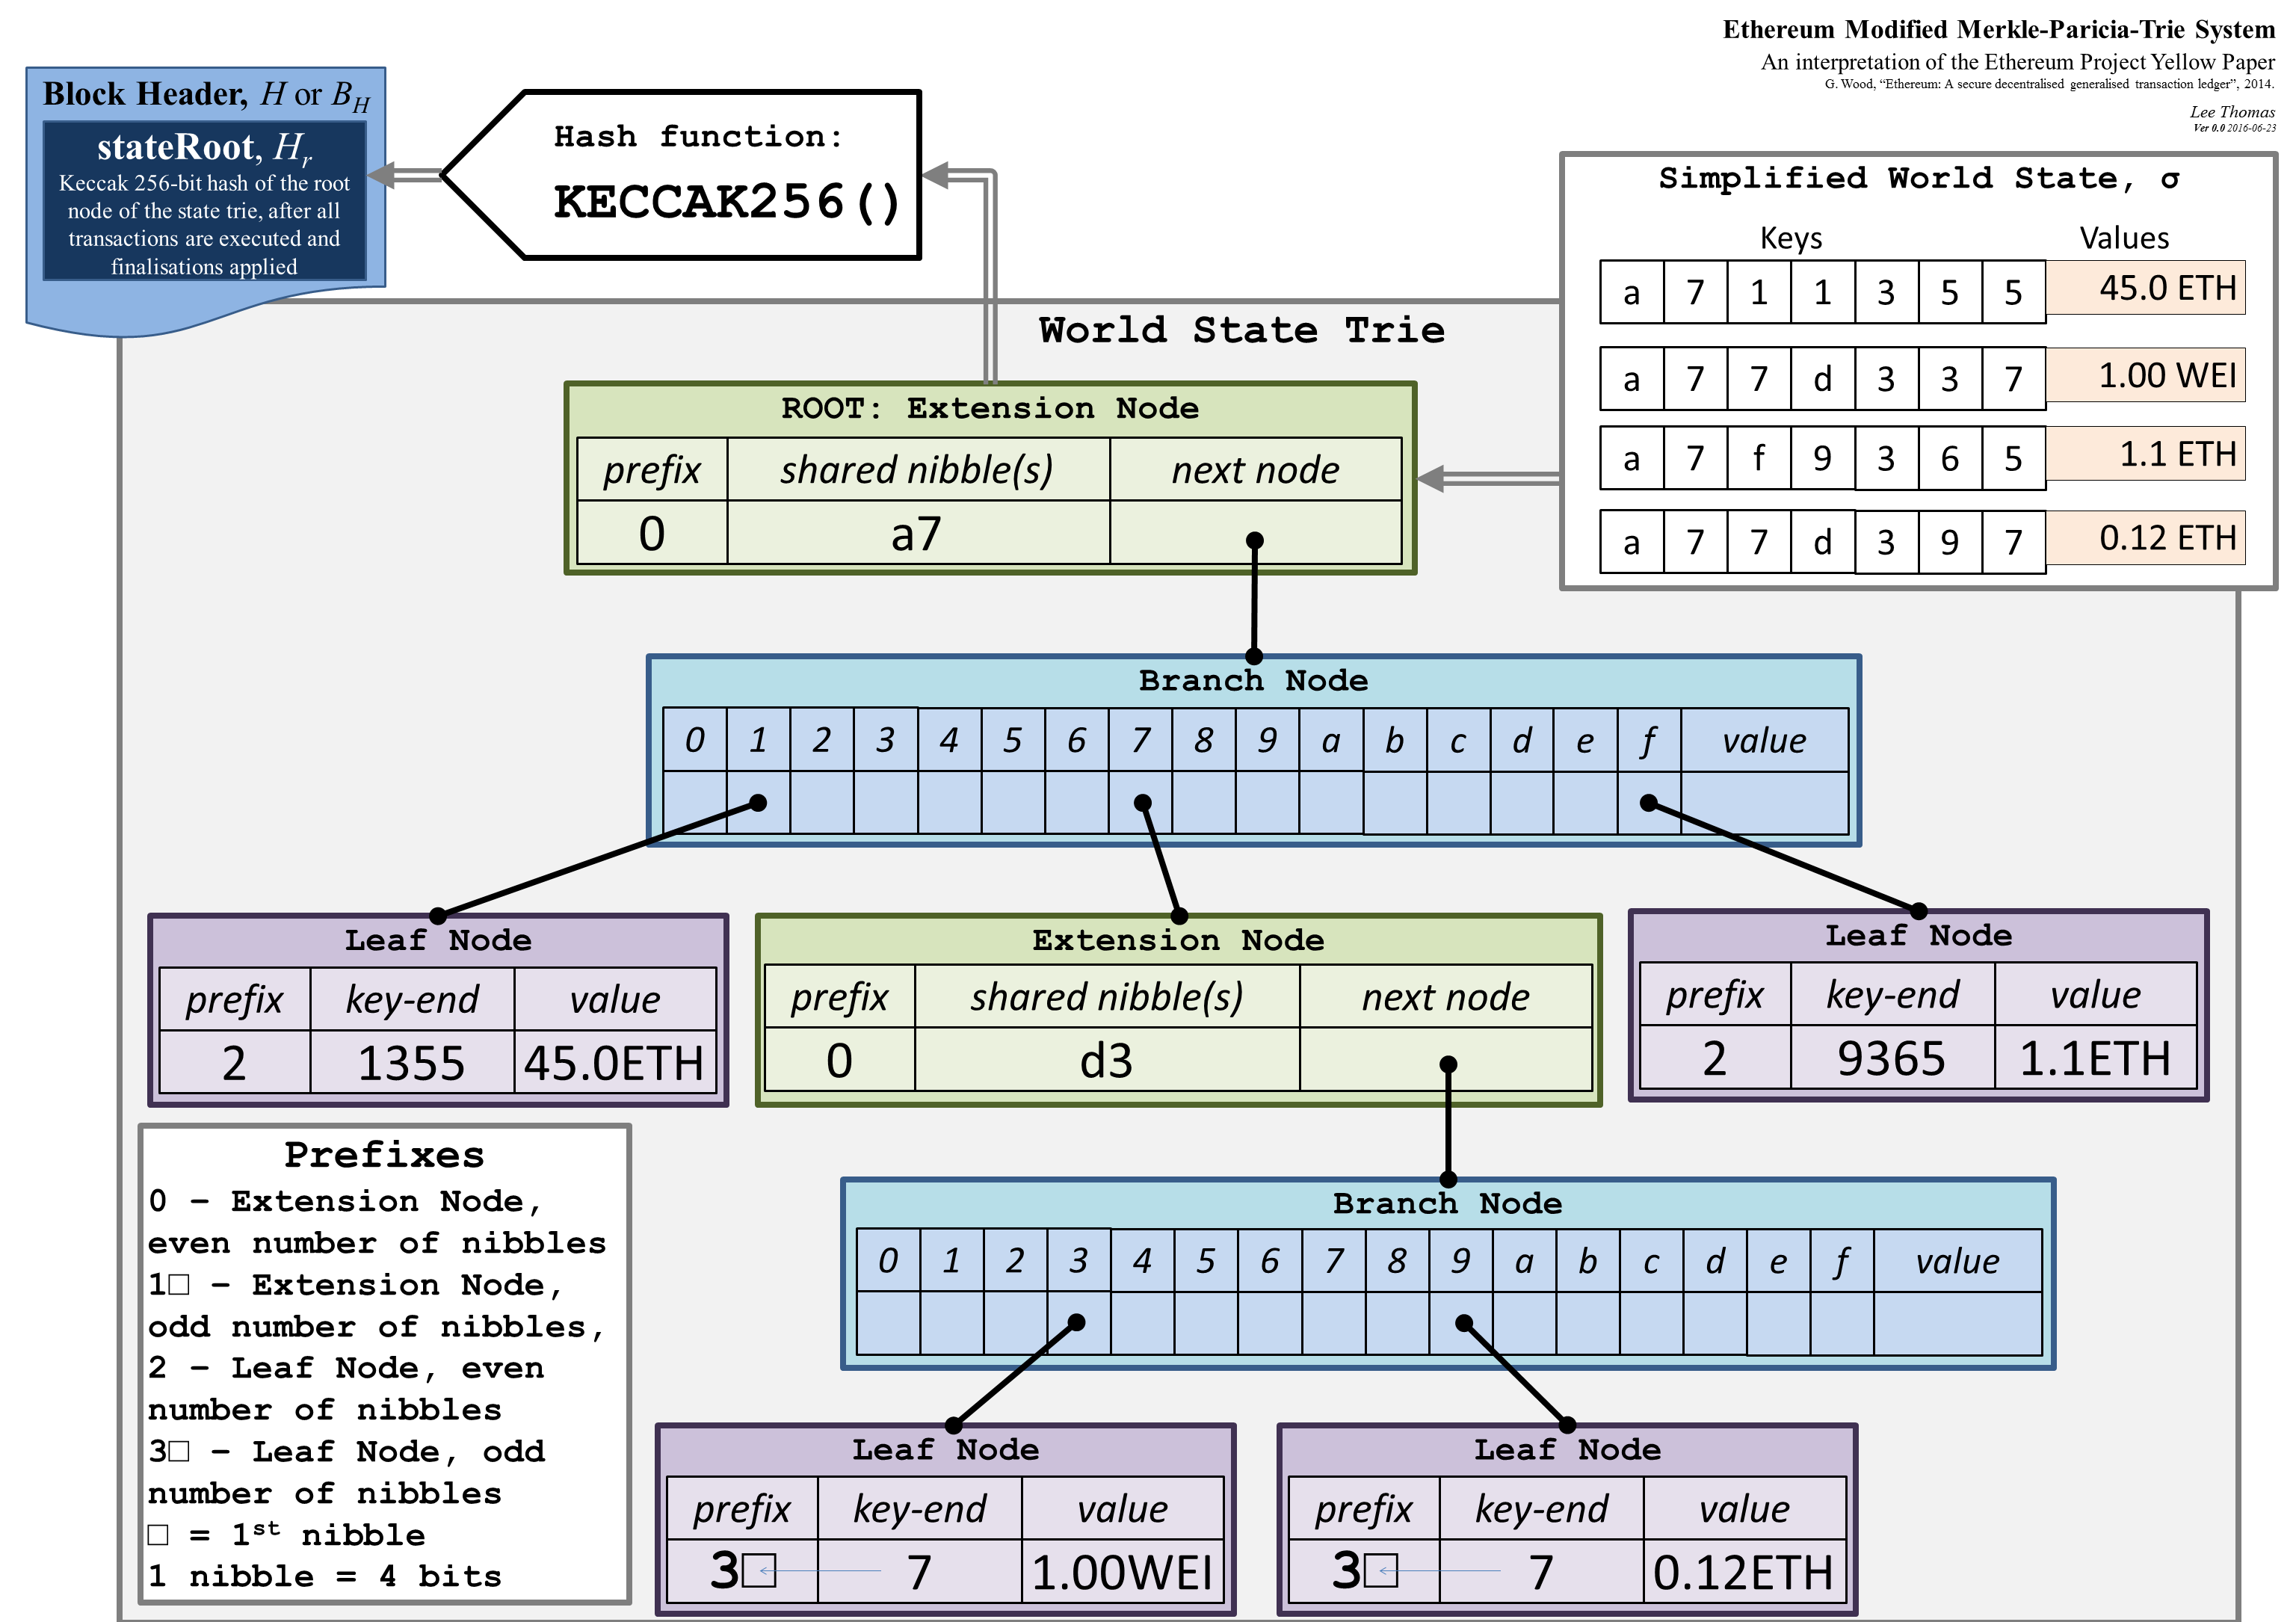
\includegraphics[width=0.9\linewidth]{background/ethereum_mpt.png}
    \caption{Ethereum patricia tree}
    \label{fig:eth_mpt}
\end{figure}

The Patricia merkle tree used in Ethereum modifies the original Patricia tree. The keys are hexadecimal strings and defines 4 types of nodes: 
\begin{itemize}
    \item EmptyNode represented as the empty string
    \item BranchNode: a 17-item node [ v0 ... v15, vt ]
    \item LeafNode: a 2-item node [ encodedPath, value ]
    \item ExtensionNode: a 2-item node [ encodedPath, key ]
\end{itemize}
A branch node at a certain step t, at letter t, is created when there are multiple possible letters for the next letter at $t+1$. Since we use hexadecimal keys, at each step we can choose between 16 letters (or the value).

A leaf node is the last possible node in the branch and contains the value. Here we can say that the key represents the adress of the ethereum account and the value is the balance. 

The extension node is the compression offered by the Patricia trie. It represents the shared nibbles (letter) before two or more words diverge. 



Ethereum\cite{Buterin..13} stores three merkle roots in the block header. One for the transactions as in bitcoin, another one for the state (balances for example), and another one for the receipts. 


\section{Zero knowledge}
\label{zeroknowledge}
This is meant to be a light introduction to the zero knowledge proof concept to understand the following interoperability solutions. 

A zero-knowledge protocol is a method by which one party (the prover) can prove to another party (the verifier) that something is true, without revealing any information apart from the fact that this specific statement is true. \cite{Goldwasser}

For example, in digital signature, you send a signature proving that you are indeed the one sending the mail. More precisely, this signature prove that you know the private key without revealing it. The verifier checks that the signature matches the public key of the sender. ( $\sim$ signature reveals the public key)
\\Instead of only proving that you know the private key as in digital signatures, zero knowledge proofs can prove "any type" of computation. 
\\For example, you can prove that: 
\begin{itemize}
    \item you know m when you send H=SHA3(m) to the verifier, without revealing m. 
    \item you know a sudoku solution to a sudoku problem without revealing it 
    \item you know the $1000^{th}$ fibonacci number ( $a_{n-2}+a_{n-1}=a_n$)
    \item the transactions are valid. This allow the ZK roll-ups to process the transactions off chain, and prove on chain to layer 1 that these transactions are indeed valid. 
\end{itemize}

In fact, zero knowledge proofs allow two properties. 

\textbf{Computational integrity} prove that you have done the right computation, even when no one is watching. For example, in ZK-rollups the computational integrity is the main need and the privacy is not always/often taken into account. 

\textbf{Privacy} with zero knowledge, you don't reveal anything about the statement. In Zerocash\cite{sasson2014zerocash}, the privacy is needed to ensure the confidentiality of the transactions. 


\paragraph{} A zero knowledge protocol should verify:
\begin{itemize}
    \item \textbf{Completeness}: If the claim is valid, the verifier accepts the proof.
\item \textbf{Soundness}: If the claim is invalid, the verifier should reject the proof with very high probability.

\item \textbf{Zero-knowledge}: The verifier learns nothing about a statement beyond its validity or falsity 
\end{itemize}

To conclude, some important properties are expected from these protocols. We want of short proof in terms of size for example. We also want, and this is a fundamental requirement, a very fast verification. If the prover with a highly efficient computer computes the hash of a 200GB document, the verification should be very fast and consists in a much lighter computation than the prover one.

This last requirement is at the heart of the zero knowledge research and explains the complexity of the techniques used.